%%%%%%%%%%%%%%%%%%%%%%%%%%%%%%%%%%%%%%%%%%%%%%%%%%%%%%%%%%%%%%%%%%% 
%                                                                 %
%                            CHAPTER THREE                         %
%                                                                 %
%%%%%%%%%%%%%%%%%%%%%%%%%%%%%%%%%%%%%%%%%%%%%%%%%%%%%%%%%%%%%%%%%%% 
 
\chapter{MATRIX-FREE SOLUTION OF THE LINEAR SYSTEMS}\label{chap:linsys}
During the execution of Algorithm~\ref{alg:pc}, the tangent linear system and
Newton update are solved many times.  Therefore, in order for the
predictor-corrector algorithm to be competitive, these systems must be
(inexactly) solved with high efficiency.  Both systems, \eqref{eq:predictorx}
and \eqref{eq:cor}, take the form
\begin{equation}\label{eq:linsys}
  (\nabla_q H) x = b,
\end{equation}
where $b \in
\mathbb{R}^{N}$ is either $F - G$, in the case \eqref{eq:predictorx} for the predictor step or $-H$ in the case of \eqref{eq:cor} for a corrector step.  We inexactly solve these systems using a preconditioned
Krylov-iterative method.  The primary challenge with this approach, as discussed
in Chapter~\ref{chap:1}, is that the preconditioner itself must be matrix free.

To address this requirement, a matrix-free preconditioner has been proposed as part of this thesis. 
The bulk of this chapter focuses on describing the matrix-free preconditioner and exercising it on some numerical experiments.  However, we begin with a brief review of the Krylov iterative solver that needs the preconditioner.

\section{Krylov Iterative Solver}\label{2:krylov}
We use the flexible generalized minimal residual method,
FGMRES~\cite{Saad1993fgmres}, to solve~\eqref{eq:linsys}.  One advantage of
FGMRES, compared to most Krylov-based methods, is that it permits nonstationary
preconditioners that vary from one Krylov iteration to the next.  While we do
not take advantage of nonstationary preconditioners in this work, we have found
this flexibility invaluable in the solution of multidisciplinary optimization
problems~\cite{dener:idf2017, dener:2014}.

To find an approximate solution to \eqref{eq:linsys}, FGMRES orthonormalizes a
sequence of matrix-vector products using a generalized form of Arnoldi's
method~\cite{saad:2003}.  Starting with $v_{1} = b/\|b\|$, the generalized
Arnoldi's method produces the following relation at the $i$th iteration:
\begin{equation}\label{eq:arnoldi}
  (\nabla_q F) \mat{Z}_{i} = \mat{V}_{i+1} \bar{\mat{H}}_{i},
\end{equation}
where $\mat{V}_{i+1} \in \mathbb{R}^{N\times (i+1)}$ has orthogonal columns and
$\bar{\mat{H}}_{i} \in \mathbb{R}^{(i+1)\times i}$ is upper Hessenberg.  The
vectors in $\mat{Z}_{i} \in \mathbb{R}^{N\times i}$ form the subspace from which
the approximate solution to \eqref{eq:linsys} is drawn (see below).  These
vectors are related to the vectors in $\mat{V}_{i+1}$ by
\begin{equation*}
  z_{j} = P_j(v_{j}), \qquad \forall j = 1,2,\ldots,i,
\end{equation*}
where $P_j(\cdot)$ denotes the preconditioning operation at iteration $j$.    

The FGMRES solution is given by $x_{i} = \mat{Z}_{i} y_{i}$, where $y_{i}$ is
chosen to minimize the 2-norm of the residual, $r_i \equiv b -  (\nabla_q F) x_i = b -  (\nabla_q F)\mat{Z}_i y_i$. The solution to this minimization problem is 
\begin{align*}
  y_{i} = \underset{y \in \mathbb{R}^i}{\textrm{argmin}}
  \lVert b -  (\nabla_q F) \mat{Z}_i y \| 
  &= \underset{y \in \mathbb{R}^i}{\textrm{argmin}}
  \lVert \mat{V}_{i+1} (\|b\| e_1 - \bar{\mat{H}}_{i} y) \| \\
  &= \underset{y \in \mathbb{R}^i}{\textrm{argmin}}
  \lVert \|b\| e_1 - \bar{\mat{H}}_{i} y \|,
  \qquad\qquad\text{(since $\mat{V}_{i+1}^T \mat{V}_{i+1} = \mat{I}$)}
\end{align*}
where $e_{1} \in \mathbb{R}^{i+1}$ is the first column of the $(i+1)\times(i+1)$
identity. The least-squares minimization problem on the final line is inexpensive to solve 
in our applications,  since $i$ is usually less than 100.

Like most Krylov iterative methods, the FGMRES algorithm described above does
not require the Jacobian $(\nabla_q F)$ explicitly.  From the user's
perspective, the algorithm only requires matrix-vector products and
preconditioning operations.  In this work, matrix-vector products involving
$(\nabla_q F)$ are computed using second-order adjoints~\cite{wang:1992,
  hicken:inexact2014}.  Briefly, each product with $(\nabla_q F)$ requires the
solution of two discretized linear PDEs: a linear forward problem and a linear
adjoint problem.  See \cite{dener:scitech2015} for further details regarding
second-order adjoints in the context of reduced-space problems with state
constraints.  The second required operation, preconditioning, is described in
subsection~\ref{sec:matfreepc}.


\section{Review on Preconditioners for Optimization}\label{2:krylov:pc}
Using Krylov methods to solve the linear systems saves the effort of computing and storing the constraint Jacobian and Lagrangian Hessian, but the convergence rate of Krylov solvers depends on the distribution 
of the system's eigenvalues. If the eigenvalues are clustered in a small radius, the convergence rate is 
generally better, and poor convergence often arises 
when the ratio of the largest to the smallest eigenvalue modulus is large, \eg $10^5$ to $10^9$. 

%In the context of the PDE-constrained optimization problem, there are two sources of ill-condition. The first one resides in PDE solvers. When the discretization is refined, some of the eigenvalues of the PDE system matrix could go towards zero. This is also called an ill-posed PDE problem. The second source of ill-condition often arises from optimization algorithms themselves. For example in the interior-point method family, the slack variables are used to measure the activeness of the inequality constraints. When some of the inequality constraints get close to the boundary, the corresponding slack variables would approach zero, and some entries on the diagonal of the KKT matrix will go unbounded. The second type of ill-condition is the target in this thesis, as the first type is usually covered as part of the PDE solver.     

In the presence of ill-conditioning, a nonsingular matrix can transform the linear system to a better conditioned one with the same solutions. This nonsingular matrix is called the preconditioner, and it exists in the form of mathematical operations in matrix-free methods. 
A preconditioner is an operator that is designed to cluster a system's eigenvalues;  
it usually does this indirectly by approximating the action of the matrix inverse and should be inexpensive to apply.  When the preconditioner is stationary, it can be represented as a matrix $P \in \mathbb{R}^{N\times N}$.  Thus, in the present case we would like
\begin{equation*}
P_j(u) \approx (\nabla_q H)^{-1}u                        %P v \approx (\nabla_q H)^{-1},
\end{equation*}
in some sense where $u \in \mathbb{R}^{N}$ is arbitrary. 


Many general preconditioners have been developed for saddle-point 
problems\\~\cite{benzi2005numerical}, such as incomplete LU factorizations~\cite{BENZI2002418, NLA:NLA320, saad:2003}, incomplete null-space factorization~\cite{nullspace_precond, 2015arXiv151106845L}, and approximate Schur complement decompositions~\cite{Bergamaschi2004, DBLP:journals/corr/LiXS15}. 
These preconditioners all involve direct operations to the entries of the system matrix, which would be infeasible for matrix-free methods. Furthermore, the diagonal entries of the system matrix in interior-point type optimizations could approach zero or infinity for inequality constraints, causing linear algebraic error in direct factorization methods. 

In addition, many specialized preconditioners have been investigated for full-space PDE-constrained optimization; see, for example,~\cite{Rees2010optimal}.
However, most full-space PDE-constrained optimization preconditioners also rely on
the availability of a matrix-based preconditioner for the state Jacobian. There
is no analogous matrix-based preconditioners for the total Jacobian $\nabla_x g$
in the reduced-space, and, as explained in Chapter~\ref{chap:1}, forming $\nabla_x
g$ explicitly is not feasible. In the making of this thesis, a Uzawa type 
preconditioner~\cite{Hu_uzawa} has been investigated but without success. 
The preconditioner proposed in this thesis is also based on the approximate Schur complement decompositions. 


%Inspired by the domain-decomposed Schur preconditioners  in PDE solvers~\cite{keyes_domain} ,  where approximate subdomain solutions of the mesh field are used as preconditioners for the iterative solver of the PDEs, \cite{DBLP:journals/siamsc/BirosG05} uses approximate state and adjoint solutions in the Schur of the KKT system as the preconditioner for the linear system of the optimization problem. 
% \cite{pc_kkt_control} presented a similar KKT matrix preconditioner for  optimization in distributed control problems using an interior-point method; it decomposes the KKT matrix according to its block structures, 
%then used existing preconditioners for the PDE solvers to approximately solve the preconditioning system. However, the preconditioner is not ideal as the preconditioned system has both positive and negative eigenvalues. In addition, \cite{doi:10.1137/15M104075X} constructed a preconditioner for the full-space Lagrange-Newton method for multi-field problems. The preconditioner removes the field variables that are causing the nonlinearity of the system, resulting in a well-balanced Newton system. 

\section{Matrix-free Preconditioner}\label{sec:matfreepc}
As $\mu$ approaches zero, the system \eqref{eq:linsys} becomes an increasingly
ill-conditioned saddle-point problem.  Consequently, solving this problem with
an iterative Krylov solver, like FGMRES, requires an effective preconditioner.  
 One of the primary contributions of
this work is a matrix-free\footnote{In this context, matrix-free means that we
  do not require a matrix whose size is the same size as $\nabla_x g$; however,
  we do use low-rank matrices.} preconditioner for reduced-space PDE-constrained
optimization with state-based constraints.

 To motivate our preconditioner,
we begin by examining the exact Jacobian $\nabla_q H$ in  \eqref{eq:predictorx} and \eqref{eq:cor}:
\begin{equation}\label{eq:dHdq}
\begin{aligned}
\nabla_q H &= (1 - \mu) \nabla_{q} F(q) + \mu \nabla_q G(q,q_0) \\
&=  (1-\mu)\begin{bmatrix}
 \nabla_{xx} \mathcal{L}   & \boldsymbol{0} & \nabla_x h^T   &  \nabla_x g^T   \\   % \mathsf{A}^T_h
\boldsymbol{0}     &   - \mat{\Lambda}_g   & \boldsymbol{0} & -\mathsf{S}     \\
\nabla_x h &  \boldsymbol{0}   & \boldsymbol{0} &  \boldsymbol{0}  \\
\nabla_x g  & -\mathsf{I}  &  \boldsymbol{0}  & \boldsymbol{0}   \\
\end{bmatrix}
+ \mu \begin{bmatrix}
\mathsf{I} & \boldsymbol{0} & \boldsymbol{0} & \boldsymbol{0} \\
\boldsymbol{0}  & \mathsf{I}  & \boldsymbol{0} & \boldsymbol{0} \\
\boldsymbol{0} & \boldsymbol{0} & -\mathsf{I} &  \boldsymbol{0} \\
\boldsymbol{0} & \boldsymbol{0} &   \boldsymbol{0} & -\mathsf{I} 
\end{bmatrix} \\
& = \begin{bmatrix}
	\mat{W}_\mu & \phantom{-}\mat{0} & \phantom{-}\mat{A}_{h,\mu}^T  & \phantom{-}\mat{A}_{g,\mu}^T \\
	\mat{0}  & -\mat{\Lambda}_\mu & \phantom{-}\mat{0}   & -\mat{S}_\mu \\
	\mat{A}_{h, \mu} & \phantom{-}\mat{0} &  -\mu \mat{I} & \phantom{-}\mat{0}  \\
	\mat{A}_{g, \mu} & -(1-\mu)\mat{I} &  \phantom{-}\mat{0}     &   -\mu \mat{I}
\end{bmatrix}
\end{aligned}
\end{equation}
where $\mat{I}$ is the identity matrix, whose size can be inferred from the context; 
and the sub-Jacobians are defined by
\begin{gather*}
	\mat{W}_{\mu} \equiv (1-\mu) \left[\nabla_x^2 f + \lambda_h^T \nabla_x^2 h  + \lambda_g^T \nabla_x^2 g\right] + \mu \mat{I},\qquad
	\mat{A}_{h, \mu} \equiv (1-\mu) \nabla_x h, \\
	\mat{A}_{g, \mu} \equiv (1-\mu) \nabla_x g, \qquad 
	\mat{S}_{\mu} \equiv (1-\mu)\mat{S},\qquad
	\mat{\Lambda}_\mu \equiv (1-\mu)  \mat{\Lambda}_g - \mu \mat{I}. 
\end{gather*}

In the ideal case, a preconditioner application corresponds to solving the
linear system
\begin{equation}\label{eq:precond}
(\nabla_q H) v = u 
\end{equation}
for $v \in \mathbb{R}^{N}$ given an arbitrary $u \in \mathbb{R}^{N}$, where
\begin{align*}
u &=
\begin{bmatrix}
u_x^T & u_s^T & u_h^T & u_g^T \end{bmatrix}, \\
v &=
\begin{bmatrix}
v_x^T & v_s^T & v_h^T & v_g^T \end{bmatrix}, 
\end{align*}
and $u_x, v_x \in \mathbb{R}^n$, $u_s, v_s \in \mathbb{R}^{m}$,  $u_h, v_h \in
\mathbb{R}^{l}$,  and $u_g, v_g \in \mathbb{R}^{m}$.  To simplify the presentation, 
we will first consider the case when only inequality constraints are present, 
in which case the third row and column of~\eqref{eq:precond} are removed.  
Subsequently, we will reintroduce the equality constraints.


%The following subsections first derive the 
%solutions for inequality-only constrained systems, then extend to both equality and inequality 
%constrained systems. 

\subsection{Inequality-only Constrained Problems}
When only inequality constraints are present, the  linear system~\eqref{eq:precond} 
simplifies to 
\begin{equation}\label{eq:ideal_precond_ineq}
  \begin{bmatrix} 
	\mat{W}_\mu & \phantom{-}\mat{0} &  \phantom{-}\mat{A}_{g,\mu}^T \\
	\mat{0}  & -\mat{\Lambda}_\mu & -\mat{S}_\mu \\
	\mat{A}_{g,\mu} &  -(1-\mu)\mat{I} & -\mu \mat{I}
\end{bmatrix}
\begin{bmatrix} v_x \\ v_s \\ v_g \end{bmatrix} 
= 
\begin{bmatrix} u_x \\ u_s \\ u_g \end{bmatrix}.
\end{equation}
If at least one constraint is active, it is easy to show that
the lower right $2m \times 2m$ block in the above matrix will become singular as
$\mu \rightarrow 0$; however, for the moment, we consider the case $\mu > 0$ and
invert this block to express $v_s$ and $v_g$ as functions of $v_x$:
\begin{equation}\label{eq:vs_and_vlam}
  \begin{bmatrix} v_s \\ v_g \end{bmatrix}
  =
  \begin{bmatrix}
    \mat{C}_\mu^{-1} & \mat{0} \\
    \mat{0} & \mat{C}_\mu^{-1}
  \end{bmatrix}
  \begin{bmatrix}
    -\mu \mat{I} & \mat{S}_\mu \\
    (1-\mu)\mat{I} & -\mat{\Lambda}_\mu 
  \end{bmatrix}
  \begin{bmatrix} u_s \\ u_g - \mat{A}_{g, \mu} v_x \end{bmatrix},
\end{equation}
where 
\begin{equation*}
  \mat{C}_{\mu} \equiv \mu \mat{\Lambda}_\mu - (1-\mu) \mat{S}_\mu
  = \mu (1-\mu) \mat{\Lambda}_g - \mu^2 \mat{I}- (1-\mu)^2 \mat{S}
\end{equation*}
is a diagonal matrix.  Substituting the expression for $v_g$ from
\eqref{eq:vs_and_vlam} into the first row of \eqref{eq:ideal_precond_ineq}, we find
\begin{equation}\label{eq:schur}
\left[\mat{W}_\mu + \mat{A}_{g, \mu}^T \mat{C}_\mu^{-1} \mat{\Lambda}_\mu \mat{A}_{g,\mu}
  \right] v_x = u_x - \mat{A}_{g,\mu}^T \mat{C}_{\mu}^{-1} \left[(1-\mu) u_s -
  \mat{\Lambda}_\mu u_g \right].
\end{equation}
%Note that~\eqref{eq:schur} results from direct substition of~\eqref{eq:vs_and_vlam} into~\eqref{eq:ideal_precond_ineq}.

\begin{remark}
To derive~\eqref{eq:vs_and_vlam}, note that the matrices involved in the lower $2m\times 2m$ block in~\eqref{eq:ideal_precond_ineq} are all diagonal.  Consequently, we can apply the formula for the inverse of a $2\times 2$ matrix.  This yields

\begin{equation*}
\begin{bmatrix}
 -\mat{\Lambda}_\mu & -\mat{S}_\mu \\ 
 -(1-\mu)\mat{I} & -\mu \mat{I}  
\end{bmatrix}^{-1} 
= 
\begin{bmatrix}
  \mat{C}_\mu^{-1} & \mat{0} \\
    \mat{0} & \mat{C}_\mu^{-1}
  \end{bmatrix}
  \begin{bmatrix}
   -\mu \mat{I} & \mat{S}_\mu \\
    (1-\mu)\mat{I} & -\mat{\Lambda}_\mu 
  \end{bmatrix}
\end{equation*}
where $\mat{C}_\mu$ holds the determinant of each $2\times 2$ matrix on its diagonal.
\end{remark}

\begin{remark}
  Consider the case where all the inequality constraints are active.  $\mat{S}_\mu = 0$ and 
  the matrix in \eqref{eq:schur} becomes the Hessian for an
  augmented-Lagrangian-like function with linearized constraints:
  \begin{equation*}
  \begin{aligned}
    \lim_{\mu\rightarrow 0} W_{\mu} + \mat{A}_{g,\mu}^T \mat{C}_{\mu}^{-1}
    \mat{\Lambda}_\mu \mat{A}_{g,\mu} & = \nabla_x^{2} f + \lambda^T \nabla_x^2 g +
    \mat{S}^{-1}\mat{A}_g^{T} \mat{\Lambda}_g \mat{A}_g \\
    &= \nabla_x^{2} f + \lambda^T \nabla_x^2 g +
     \frac{1}{\tau_s}\mat{A}_g^{T} \mat{\Lambda}_g \mat{A}_g \\
   \end{aligned}
  \end{equation*}
  Notice that the fixed-value fraction-to-the-boundary rule applied to the slack variable in this thesis 
  would impose the value of $\tau_s$ on all slack variables.  
\end{remark}


The boundedness of the system \eqref{eq:schur} depends on the behavior of the
matrix $\mat{C}_{\mu}$.  Assuming strict complementarity, as $\mu\rightarrow 0$
we have two situations:
\begin{enumerate}
\item If the $i$th constraint is inactive at the solution, then $\lambda_{g,i} = 0$ and
  $\lim_{\mu\rightarrow 0} \left[\mat{C}_\mu^{-1} \mat{\Lambda}_\mu \right]_{ii}
  = 0$.  This has the effective of eliminating the corresponding constraint from
  the reduced system \eqref{eq:schur}.

\item If the $i$th constraint is active, then $s_i = 0$ and $\lim_{\mu\rightarrow 0}
  \left[\mat{C}_\mu^{-1} \mat{\Lambda}_\mu \right]_{ii} = \infty$.
\end{enumerate}
The first situation is desirable, since the constraint is inactive and should
not influence the step $v_x$.  The second situation is obviously undesirable;
however, the safeguards in place during the predictor-corrector phases bound the
slacks away from zero, so the inverse of $\mat{C}_{\mu}$ remains well defined in practice.
In particular, we use the fraction-to-the-boundary rule 
at the end of the predictor step and explicit clipping at the end of the corrector step to make sure 
the slack variables remain larger than $\tau_s$; see Section~\ref{sec:fraction} for details.



Having established that \eqref{eq:schur} is well defined for all iterates, we
now seek to approximately invert this system.  To this end, we replace
$\mat{W}_{\mu}$ by an approximation denoted by $\mat{B}_{\mu}$:
\begin{equation*}
\mat{W}_{\mu} \approx \mat{B}_{\mu},
\end{equation*}
where $\mat{B}_{\mu}$ is either a scaled identity, $\mat{B}_{\mu} = \beta
\mat{I}$, or an L-BFGS quasi-Newton approximation~\cite{liu:1989}.  In addition,
we use the Lanczos algorithm~\cite{saad:1992} to construct a low-rank
approximation of $\mat{A}_{g,\mu}^T \mat{C}_\mu^{-1} \mat{\Lambda}_\mu
\mat{A}_{g,\mu}$ for the nonlinear constraints; that is
\begin{equation}\label{eq:svd}
  \mat{A}_\mu^T  \mat{C}_\mu^{-1}  \mat{\Lambda}_{\mu}\mat{A}_\mu
  \approx \mat{U} \mat{\Sigma} \mat{V}^T,
\end{equation}
where $\mat{\Sigma} = \textsf{diag}(\sigma_1,\sigma_2,\ldots,\sigma_{\nsig}) \in
\mathbb{R}^{\nsig\times \nsig}$ is a diagonal matrix holding estimates for the
$\nsig$ largest singular values, and $\mat{U} \in \mathbb{R}^{m\times \nsig}$ and
$\mat{V} \in \mathbb{R}^{m\times \nsig}$ are the corresponding approximations to the
left and right singular vectors. 

\begin{remark}
  The Lanczos algorithm is advantageous in this context, because it only
  requires matrix-vector products with $\mat{A}_{g,\mu}^T \mat{C}_\mu^{-1}
  \mat{\Lambda}_\mu \mat{A}_{g,\mu}$.  Such products can be evaluated using
  second-order adjoints; see \cite{hicken:inexact2014} or
  \cite{dener:scitech2015} for further details regarding second-order adjoints.
  Furthermore, by replacing accurate second-order adjoint PDE solves with
  corresponding preconditioner applications, the cost of the Lanczos-based SVD
  can be significantly reduced.  This idea is explored in the numerical
  experiments in Chapter~\ref{chap:tests}.  
\end{remark}

%\begin{remark}
%  The constraint Jacobian for bound and linear constraints is readily available,
%  so the Lanczos algorithm is not necessary to approximate $\mat{A}_{g,\mu}^T
%  \mat{C}_\mu^{-1} \mat{\Lambda}_{\mu}\mat{A}_{g,\mu}$ in this case.
%  \todo[inline]{But the matrix $\mat{A}_\mu^T \tilde{\mat{C}}_\mu^{-1}
%    \mat{\Lambda}^{-1}\mat{A}_\mu$ involves products between the nonlinear and
%    linear constraints; how do you account for this in Lanczos?  
%   \padd{ By zeroing the corresponding portions in the middle term  $C_{\mu}*\Lambda$, 
%   the products AXA would be only for the nonlinear constraint part.   The bound constraint
%   part of AXA, which is $C_{\mu}*\Lambda$ times Identity matrix, is added to the Hessian
%   W part.  $B_{\mu}$ is the sum of the Hessian and bound constraint. 
%     }}
%\end{remark}

%\begin{remark}
% At the beginning of the homotopy iterations when the activeness of the constraints are far from 
%determined, it happens sometimes that  $ \mat{C}_\mu^{-1}  \mat{\Lambda}_{\mu}$ are close to 
%vector of zeros, resulting in rank dependent matrix-vector products in Lanczos iterations. To deal 
%with this issue, at the beginning, we use $  \mat{A}_\mu^T \mat{A}_\mu
%  \approx \mat{U} \mat{\Sigma} \mat{V}^T $ in the preconditioner at the beginning of the homotopy iteration. 
%  When $\mu$ gets smaller than $\Sigma_e$, we use \eqref{eq:svd} in the preconditioner. 	
%\end{remark}

Based on the above approximations, the (approximate) inverse of the matrix in
\eqref{eq:schur} can be found using the Sherman-Morrison-Woodbury formula as follows:
\begin{align}
\left[\mat{W}_\mu + \mat{A}_\mu^T \mat{C}_\mu^{-1}  \mat{\Lambda}_\mu  \mat{A}_\mu \right]^{-1}
&\approx
\left[\mat{B}_{\mu} + \mat{U} \mat{\Sigma} \mat{V}^T \right]^{-1} \notag \\
&= \mat{B}_\mu^{-1} - \mat{B}_\mu^{-1} \mat{U}  \left(  \mat{I}_{\nsig} +  \mat{\Sigma} \mat{V}^{T} \mat{B}_\mu^{-1} 
\mat{U} \right)^{-1} \mat{\Sigma} \mat{V}^{T} \mat{B}_\mu^{-1},
\label{eq:smw}
\end{align}
where $\mat{B}_\mu^{-1}$ is either $(1/\beta)\mat{I}$ or the L-BFGS
approximation.  Note that, in the above expression, $\left(\mat{I}_{\nsig} +
\mat{\Sigma} \mat{V}^{T} \mat{B}_{\mu}^{-1} \mat{U} \right)$ is an $\nsig\times
\nsig$ matrix.  In the proposed preconditioner, we assume that the number of
singular values in the truncated SVD, \ie $\nsig$, is sufficiently small that we
can invert this matrix explicitly using an $LU$ factorization.

In summary, to approximately solve \eqref{eq:schur} we evaluate
\begin{equation}\label{eq:vx}
  v_x = \left[\mat{B}_\mu^{-1} - \mat{B}_\mu^{-1} \mat{U}  \left(  \mat{I}_{\nsig} +  \mat{\Sigma} \mat{V}^{T} 
  \mat{B}_\mu^{-1} \mat{U} \right)^{-1} \mat{\Sigma} \mat{V}^{T} \mat{B}_\mu^{-1} \right]
  \left\{ u_x - \mat{A}_\mu^T \mat{C}_{\mu}^{-1} \left[(1-\mu) u_s -
  \mat{\Lambda}_\mu u_g \right]\right\}.
\end{equation}
After obtaining $v_x$, we use it in \eqref{eq:vs_and_vlam} to
find $v_s$ and $v_\lambda$;
\begin{align}
  v_s &= \mat{C}_\mu^{-1}\left[-\mu u_s + \mat{S}_\mu \left( u_g - \mat{A}_\mu v_x\right) \right], \label{eq:vs} \\
  v_\lambda &= \mat{C}_\mu^{-1}\left[(1-\mu)u_s - \mat{\Lambda}_\mu \left( u_\lambda - \mat{A}_\mu v_x \right) \right]. 
  \label{eq:vlam}
\end{align}


We conclude this section by summarizing the inequality-only matrix-free preconditioner
in Algorithm~\ref{alg:precond}.  Note that the approximate SVD can be performed
before each Krylov iterative solve, or it can be performed periodically to
reduce cost, possibly at the risk of descreasing the effectiveness of the
preconditioner.

\LinesNumberedHidden
\begin{algorithm}[tbp]\setstretch{1.35}
\SetKwInOut{Input}{Input}
\SetKwInOut{Output}{Output}
\SetKwInOut{Parameter}{Parameters}
\SetKw{Return}{return}
\SetEndCharOfAlgoLine{}

\Parameter{values at which to evaluate matrices, $x$, $s$,  $\lambda_g$, and $\mu$};  $\nsig$
 
\Input{vectors to precondition, $u_x$, $u_s$, $u_{\lambda_g}$}
\Output{preconditioned vectors, $v_x$, $v_s$, $v_{\lambda_g}$}
\BlankLine
Build the truncated and approximate SVD \eqref{eq:svd}, using 
preconditioner applications in place of exact second-order adjoint solves \\
Solve for $v_x$ using \eqref{eq:vx}\\
Solve for $v_s$ using \eqref{eq:vs}\\
Solve for $v_{\lambda_g}$ using \eqref{eq:vlam}\\
\Return $v_x$, $v_s$, and $v_{\lambda_g}$
\caption{Matrix-free, approximate SVD preconditioner. \label{alg:precond}}
\end{algorithm}

\subsection{Preconditioner for Problems with both Inequality and Equality Constraints}
%it is not obvious to reduce the system in 
%\eqref{eq:ideal_precond} using the Schur complement method.
When both equality and inequality constraints are present, it is straightforward 
to extend the preconditioner to handle the general 
constrained case, since the 
equality-constraint rows in~\eqref{eq:precond} do not involve $v_s$ or $v_g$.
Indeed, in the general case the reduced system becomes
\begin{equation}\label{eq:schur_equ2}
\begin{bmatrix}
\mat{W}_\mu +  \mat{A}_{g,\mu}^T  \mat{C}_\mu^{-1} \mat{\Lambda}_\mu    \mat{A}_{g,\mu}    & \mat{A}_{h,\mu}^T   \\
\mat{A}_{h,\mu}  & -\mu \mat{I}
\end{bmatrix}
\begin{bmatrix} v_x \\ v_h  \end{bmatrix} 
=
\begin{bmatrix} u_x - \mat{A}_{g,\mu}^T \mat{C}_\mu^{-1}  \left[(1-\mu) u_s  - \mat{\Lambda}_\mu u_g     \right]  \\ u_h  \end{bmatrix}. 
\end{equation}
When both equality and inequality constraints present, we need to solve \eqref{eq:schur_equ2} rather than~\eqref{eq:schur}. Subsequently,  $v_s$ and $v_g$ can be recovered by \eqref{eq:vs_and_vlam} the same way as in the inequality-only case. Thus, the problem becomes how to solve \eqref{eq:schur_equ2} 
 using matrix-free methods. Once again we take advantage of the Schur complement. 
%\begin{equation}\label{eq:reduce}
%\begin{bmatrix}
%\mat{W}_\mu +  \mat{A}_{g,\mu}^T  \mat{C}_\mu^{-1} \mat{\Lambda}_\mu  \mat{A}_{g,\mu}    & \mat{A}_{h,\mu}^T   \\
%\mat{A}_{h,\mu}  & -\mu \mat{I}
%\end{bmatrix}
%\begin{bmatrix} v_x \\ v_h  \end{bmatrix} 
%=
%\begin{bmatrix} \hat{u}_x   \\ u_h  \end{bmatrix} 
%\end{equation}
%Note that the first row in the right-hand-side of \eqref{eq:schur_equ2} is denoted by $\hat{u}_x$ in \eqref{eq:reduce}.  

Recall that, if $\mat{D}$ and $\left( A-BD^{-1}C \right) $ are invertible,  
then the solution of the linear system 
\begin{equation*}
\begin{bmatrix}
\mat{A}  & \mat{B} \\
\mat{C}  & \mat{D} 
\end{bmatrix} 
\begin{bmatrix}
x \\ y
\end{bmatrix}
= 
\begin{bmatrix}
a \\ b
\end{bmatrix}, 
\end{equation*}
is given by, 
\begin{equation}\label{eq:schur_inv}
\begin{bmatrix}
x \\ y
\end{bmatrix}=
\begin{bmatrix}
I  & 0 \\
-D^{-1}C  & I 
\end{bmatrix}
 \begin{bmatrix}
\left( A-BD^{-1}C \right)^{-1}   &  0 \\
 0   & D^{-1} 
\end{bmatrix}
\begin{bmatrix}
I  &   -BD^{-1} \\
0  &  I 
\end{bmatrix}
\begin{bmatrix}
a \\ b
\end{bmatrix}
\end{equation}


To use the above factorization in~\eqref{eq:schur_equ2}, we have to consider two situations: 
\begin{enumerate}
\item When $\mu$ is not small, \eg $\mu > \tau_{\mu}$, then $- \mu \mat{I}$ is invertible and we can use \eqref{eq:schur_inv}.   %, $\bar{\mu} =  \mu$. 
\item When $\mu$ gets close to zero, \eg $\mu < \tau_{\mu}$, we enforce the clipping rule 
$ \bar{\mu} = \max(\mu, \tau_\mu) $ 
to prevent $\mu$ from being too small in the preconditioner. We use $\tau_{\mu} = 10^{-4}$ for all the numerical experiments in this work. With this safeguard,  \eqref{eq:schur_inv} can still be used as a preconditioner.
\end{enumerate}
To summarize, in the general constrained case, $v_x$ and $v_h$ can be obtained as follows:
\begin{equation}\label{eq:core_equ}
\begin{bmatrix} v_x \\ v_h  \end{bmatrix} 
=
\begin{bmatrix}
I & 0 \\
\frac{1}{\bar{\mu}} \mat{A}_{h,\mu}  &  I 
\end{bmatrix}
\begin{bmatrix}
\left(\mat{W}_\mu +  \mat{A}_{g,\mu}^T  \mat{C}_\mu^{-1} \mat{\Lambda}_\mu  \mat{A}_{g,\mu}  
+ \frac{1}{\bar{\mu}}  \mat{A}_{h,\mu}^T \mat{A}_{h,\mu} \right)^{-1}    & 0 \\
0  &  -\frac{1}{\bar{\mu}}\mat{I} 
\end{bmatrix}
\begin{bmatrix}
I  & \frac{1}{\bar{\mu}} \mat{A}_{h,\mu}^T  \\
0  &  I
\end{bmatrix}
\begin{bmatrix}
\hat{u}_{x} \\ u_h
\end{bmatrix},
\end{equation}
where $\hat{u}_x$ denotes the $x$-component of the right-hand side of~\eqref{eq:schur_equ2}.  The most involved operation in~\eqref{eq:core_equ} is the application of the inverse Schur complelement:
\begin{equation}
\left(\mat{W}_\mu +  \mat{A}_{g,\mu}^T  \mat{C}_\mu^{-1} \mat{\Lambda}_\mu  \mat{A}_{g,\mu}  
+ \frac{1}{\bar{\mu}}  \mat{A}_{h,\mu}^T \mat{A}_{h,\mu} \right)^{-1}  \left(\hat{u}_{x} + \frac{1}{\bar{\mu}} \mat{A}_{h,\mu}^T u_{h}  \right). 
\end{equation}
%where $y$ refers to 
%\begin{equation}
%y = \text{rhs} + \frac{1}{\mu} \mat{A}_{h,\mu}^T u_h
%\end{equation}
By stacking $ \mat{A}_{h,\mu} $ and $\mat{A}_{g,\mu}$ together, 
the Schur complement can be expressed as
\begin{equation}\label{pc:eq1}
\mat{W}_\mu  +  \mat{A}_\mu ^T \Sigma_{\mu} \mat{A}_\mu = 
\mat{W}_\mu +  \mat{A}_{g,\mu}^T  \mat{C}_\mu^{-1} \mat{\Lambda}_\mu  \mat{A}_{g,\mu}  
+ \frac{1}{\bar{\mu}}  \mat{A}_{h,\mu}^T \mat{A}_{h,\mu}, 
\end{equation}
where 
\begin{equation}\label{pc:eq2}
 \mat{A}_\mu = 
 \begin{bmatrix}
 \mat{A}_{h,\mu} \\
 \mat{A}_{g,\mu}
 \end{bmatrix} \qquad\text{and}\qquad
  \Sigma_{\mu} = 
  \begin{bmatrix}  
  \frac{1}{\bar{\mu}} \mat{I}  & 0 \\
  0   &  \mat{C}_\mu^{-1} \mat{\Lambda}_\mu 
  \end{bmatrix}.
\end{equation}
Inspecting~\eqref{pc:eq1}, we see that it has the same form as the matrix on the left-hand side of~\eqref{eq:smw}.  Therefore, as before, we use the Lanczos method to construct an approximate singular-value decomposition of $\mat{A}_\mu^T \mat{\Sigma}_\mu \mat{A}_\mu$, and replace $\mat{W}_{\mu}$ with a diagonal or quasi-Newton approximation.  Subsequently, we can use the Sherman-Morrison-Woodbury formula to invert the approximation in the same manner as in the previous section. 

\section{Scalable Quadratic Optimization Problem}
\subsection{Problem Description}
We conclude this chapter with a numerical experiment to test the effectiveness of the approximate SVD
preconditioner defined in Algorithm~\ref{alg:precond}.  In particular, we are
interested in the performance of the algorithm with the preconditioner as the size of the problem increases.  
To this end, we consider the following scalable optimization problem
in which we can independently control the size and conditioning of the Hessian
and constraint Jacobian:
\begin{equation}\label{eq:quadra}
  \begin{aligned}
    \underset{x \in R^n} {\text{min}}  
     & \quad \frac{1}{2}x^T \mat{Q} x + g^T x \\
    \text{subject to}  & \quad \mat{A}x \geq b.  \\
  \end{aligned}.
\end{equation}
The vector $g\in \mathbb{R}^{n}$ is randomly sampled from a uniform distribution 
on $[ 0,1)$, while $b \in \mathbb{R}^{n}$ is randomly sampled from $[0,0.1)$. 

The Hessian $\mat{Q}$ is diagonal with entries
\begin{equation*}
  \mat{Q}_{ii} = \begin{cases}
    \frac{1}{i}, &  i = 1, 2, ...,  \kappa, \\
    \frac{1}{\kappa}, & i =  \kappa+1, ... , n, \\
  \end{cases}
\end{equation*}
where $\kappa \leq n$.  This definition produces a Hessian with a condition
number of $\kappa$,  so that its condition number 
can be controlled independently of the problem dimension.

The constraint Jacobian $\mat{A} \in \mathbb{R}^{n\times n}$ is constructed as follows. First, a diagonal matrix 
$\mat{D} \in \mathbb{R}^{n\times n}$ of singular values is defined similar to $\mat{Q}$:
\begin{equation*}
  \mat{D}_{ii} = \begin{cases}
    \frac{1}{i^2}, &  i = 1,2,...,\nu, \\
    \frac{1}{\nu^2}, & i = \nu+1, ..., n, \\
  \end{cases}
\end{equation*}
where $\nu \leq n$.  Next, matrices $\mat{A}_L  \in \mathbb{R}^{n\times n} $ and $\mat{A}_R \in \mathbb{R}^{n\times n}$ of random integers from 
the discrete uniform distribution on the
interval [0,10),  are factorized using a QR decomposition:  
\begin{equation*}
\begin{aligned}
\mat{A}_L &= \mat{Q}_L \mat{R}_L, \\
\mat{A}_R &= \mat{Q}_R \mat{R}_R. \\
\end{aligned}
\end{equation*}
Finally, the constraint Jacobian is formed as $\mat{A} =\mat{Q}_L  \mat{D} \mat{Q}_R $.  
Consequently, based on this construction, the condition number of $\mat{A}$ is $\nu ^2$ and is also controllable independent of the problem dimension.

For this study we set $\kappa = \nu = 9$, which gives condition numbers of  
$ \text{cond} (\mat{Q} )= 9$,  $ \text{cond} (\mat{A}) = 81$. 
While these are modest, even small condition numbers, we emphasize that the conditioning of the KKT matrix $\nabla_q F$ remains high, between $10^4$ and $10^9$.

%The modest condition number of 
%$\mat{Q} $ and $\mat{A}$ is benefit to our study in that we can shift 
%the focus to treat the ill-condition in the KKT matrix 
%$\nabla_{q} F(q)$ at $\mu<\epsilon_{\mu}$, whose typical condition number ranges from $10^4$ to $10^9$
%depends on the problem.

%The values of $\kappa$ and $\nu$ are chosen to be a fixed positive
%value smaller than the number of design variables.  This is to make the
%condition number of the matrix fixed, not hugely increasing with the
%dimension of the problem.

\begin{remark}
Although the matrices for this synthetic problem are available explicitly, our
algorithm does not exploit this and remains matrix-free, \ie it only uses
matrix-vector products.
\end{remark}

\subsection{Results}
We consider two problems sizes, $n=200$ and $n=500$. Figure~\ref{fig:quad_hist} plots the absolute optimality, complementarity and feasibility
histories versus CPU time. 
The predictor-corrector algorithm is applied both with and without the preconditioner.  
In addition, the plots include the results
from SNOPT~\cite{gill:2002}, a well-validated active-set SQP
optimization library.

Without the preconditioner, the predictor-corrector algorithm is not competitive
and does not converge within the time shown.  This illustrates the need for preconditioning Newton-Krylov
optmization algorithms, even for modest sized problems.  The results
also indicate that the proposed algorithm is competitive with SNOPT when $n=200$ and the proposed algorithm outperforms SNOPT when $n=500$. In both cases, the feasibility of SNOPT sharply 
decreases once when the correct set of active constraints are determined. It is notable that when  $n=500$, SNOPT takes significantly longer time than the new algorithm to converge. 
%When $n=200$, SNOPT is able to establish feasiblity within the same time as the
%predictor-corrector algorithm, but it takes significantly longer to converge the
%first-order optimality conditions.

\begin{figure}[tbp]
  \centering
  \subfloat[$n=200$\label{fig:quad_200}]{
   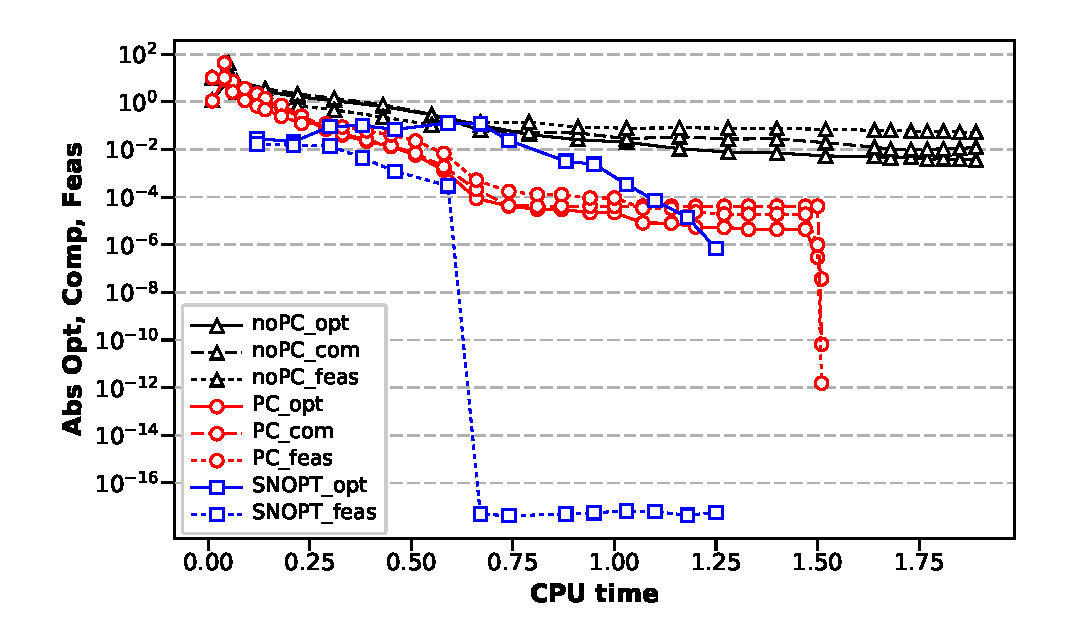
\includegraphics[clip,width=1.0\linewidth]{./figs/chap4_test/quadratic_200_color.eps} }
   \hspace{1em}
   \subfloat[$n=500$\label{fig:quad_500}]{
   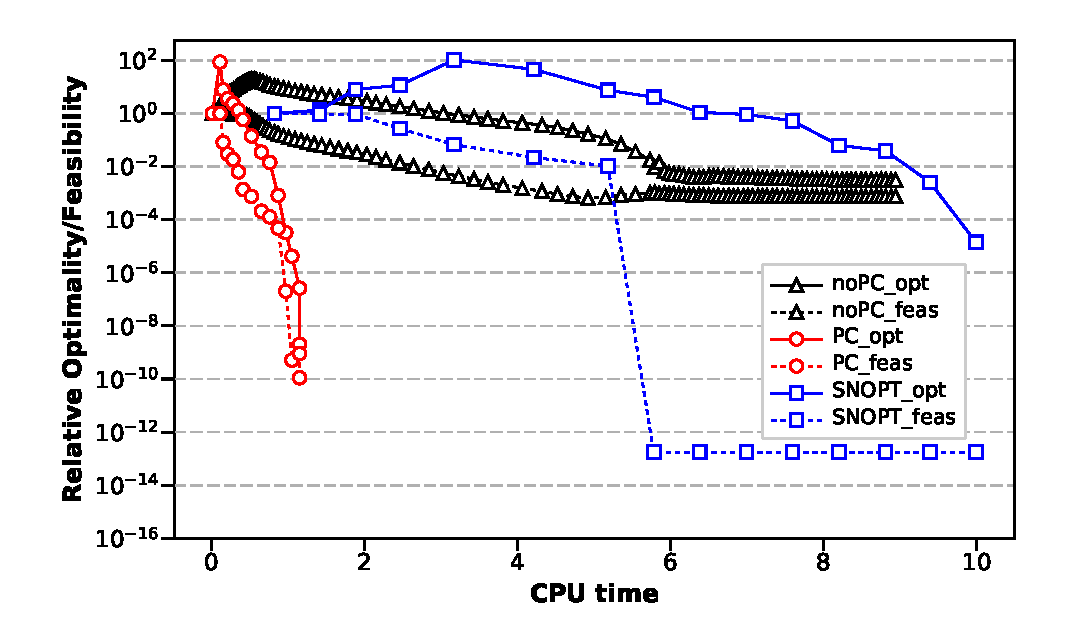
\includegraphics[clip,width=1.0\linewidth]{./figs/chap4_test/quadratic_500_color.eps} }
   \caption{Convergence histories for the scalable quadratic problem with $n=200$ and
  $n=500$. The results for the proposed algorithm, with and without
  preconditioning, are plotted together with the results from
  SNOPT.\label{fig:quad_hist}}
\end{figure}

To further explore the scalability of the proposed algorithm, we ran 100 random cases for 
each fixed sized problem, for $n = 100, 200, 300, 400, 500$.  In each random sample, the gradient 
of the objective function $g$, and the right hand side vector $b$ in the linear constraint in \eqref{eq:quadra} 
were randomly generated as described earlier. The diagonal matrices $\mat{Q}$ and $\mat{D}$ remain fixed, while $\mat{A}_L$ and $\mat{A}_R$ are randomly generated. Thus the constraint Jacobian $\mat{A}$ 
also varies for each case. 
The starting point for each run is also randomly generated. Figure~\ref{fig:quad_scale} shows the two standard deviations in time while
the problem size increases. As can be seen, the new method exhibits good scalability relative to SNOPT. 

\begin{figure}[tbp]
  \centering
  \includegraphics[clip,width=1.0\textwidth]{./figs/chap4_test/random_100_color.eps}%
  \caption{CPU cost versus number of design variables for the quadratic
    optimization problem.\label{fig:quad_scale}}
\end{figure}

We should emphasize that the proposed SVD preconditioner is particularly effective for this synthetic problem, because it is designed in such a way that the constraint Jacobian can be approiximated effectively using the Lanzcos-based SVD approximation.
Put another way, the SVD approximation can capture the main characteristics of the matrix in~\eqref{eq:svd}. For real-world problems, the distribution of the singular values of the constraint Jacobian is unknown, and may possess an unfavorable distribution pattern for the proposed preconditioner to remain effective.

%distribution of the singular values for the constraint Jacobian is readily separable, with the largest few dominates, and there are only linear inequality constraints. 


%To derive \eqref{eq:vs_and_vlam} and \eqref{eq:schur}, the system matrix in \eqref{eq:ideal_precond_ineq} can be partitioned into a $2 \times 2$ block matrix. 
%\begin{equation}\label{eq:sch}
%\left[
%\begin{array}{c | c c} 
%	   \mat{W}_\mu   &   \phantom{-}\mat{0}  &   \phantom{-}\mat{A}_{g,\mu}^T   \\
%	   \hline
%	   \mat{0}    &   -\mat{\Lambda}_\mu & -\mat{S}_\mu \\
%	  \mat{A}_{g,\mu}     &  -(1-\mu)\mat{I} & -\mu \mat{I}   
%\end{array}  
%\right]
%\left[  \begin{array}{c} v_x \\ \hline v_s \\ v_g \end{array} \right]
%= 
%\left[ \begin{array}{c} u_x \\  \hline u_s \\ u_g \end{array} \right]
%\end{equation}
%Assuming that $\mat{D}$ is invertible, the solution of the following linear system
%\begin{equation*}
%\begin{bmatrix}
%\mat{A}  & \mat{B} \\
%\mat{C}  & \mat{D} 
%\end{bmatrix} 
%\begin{bmatrix}
%x \\ y
%\end{bmatrix}
%= 
%\begin{bmatrix}
%a \\ b
%\end{bmatrix}
%\end{equation*}
%can be obtained by: 
%\begin{equation}\label{eq:schx}
%\begin{aligned}
%\left( \mat{A} - \mat{B} \mat{D}^{-1}\mat{C}  \right)x &= a - \mat{B} \mat{D}^{-1}b \\
%\mat{C}  x +  \mat{D} y &= b 
%\end{aligned}
%\end{equation}
%Note that the inverse of the lower right block matrix in \eqref{eq:sch} is equivalent to the 
%system matrix in \eqref{eq:vs_and_vlam}. 



% However, by using a basic row block by 
%row block variable elimination method, a similar reduced system like \eqref{eq:schur} can be obtained. 
%\begin{equation}\label{eq:2}
%  \begin{bmatrix} 
%	\mat{W}_\mu & \phantom{-}\mat{0} & \phantom{-}\mat{A}_{h,\mu}^T  & \phantom{-}\mat{A}_{g,\mu}^T \\
%	\mat{0}  & -\mat{\Lambda}_\mu & \phantom{-}\mat{0}   & -\mat{S}_\mu \\
%	\mat{A}_{h, \mu} & \phantom{-}\mat{0} &  -\mu \mat{I} & \phantom{-}\mat{0}  \\
%	\mat{A}_{g, \mu} &  -(1-\mu)\mat{I} &  \phantom{-}\mat{0}     &   -\mu \mat{I}
%\end{bmatrix}
%\begin{bmatrix} v_x \\ v_s \\ v_{h} \\  v_{g} \end{bmatrix} 
%= 
%\begin{bmatrix} u_x \\ u_s \\ u_{h} \\ u_{g}  \end{bmatrix},
%\end{equation}
%The slack variable $v_s$ can be represented by the inequality multipliers $v_g$ using 
%the second row block of \eqref{eq:2}: 
%% \begin{equation}
%\begin{align}
% -\mat{\Lambda}_\mu  v_s  - \mat{S}_\mu v_g  &= u_s  \notag \\
%   -v_s &=   \mat{\Lambda}_\mu ^{-1} \left[ \mat{S}_\mu v_g + u_s  \right]  
% \label{eq:vs2}
%\end{align}
%% \end{equation}
%By plugging \eqref{eq:vs2} into the last row block of \eqref{eq:2}, the inequality multiplier $v_g$ is 
%left to be represented by $v_x$ only: 
%  %\label{eq:vg}
%\begin{align}
%\mat{A}_{g,\mu} v_x -(1-\mu)\mat{I} v_s -\mu \mat{I} v_g  &= u_g  \notag \\
%\mat{A}_{g,\mu} v_x   +  (1-\mu)   \mat{\Lambda}_\mu ^{-1} \left[ \mat{S}_\mu v_g + u_s  \right] -\mu \mat{I} v_g &= u_g  \notag  \\
% v_g = \left[ (1-\mu)   \mat{\Lambda}_\mu ^{-1} \mat{S}_\mu   -\mu \mat{I} \right]^{-1} & \left[   u_g -    (1-\mu)   \mat{\Lambda}_\mu ^{-1} u_s  -   \mat{A}_{g,\mu} v_x   \right] 
% \label{eq:vg2x}
% \end{align}
%The first row block of \eqref{eq:2} can be rewritten using $v_g$ as in \eqref{eq:vg2x}:
%\begin{equation*}
% \mat{W}_\mu v_x +  \mat{A}_{h,\mu}^T v_h  + \mat{A}_{g,\mu}^T  \left[ (1-\mu)   \mat{\Lambda}_\mu ^{-1} \mat{S}_\mu   -\mu \mat{I} \right]^{-1} \left[  u_g -    (1-\mu) \mat{\Lambda}_\mu ^{-1} u_s  -   \mat{A}_{g,\mu} v_x   \right] =u_x 
% \end{equation*}
%\begin{equation*} 
%\begin{aligned}
%\left[ \mat{W}_\mu +  \mat{A}_{g,\mu}^T \left[ (1-\mu) \mat{\Lambda}_\mu ^{-1} \mat{S}_\mu   -\mu \mat{I} \right]^{-1} (-\mat{A}_{g,\mu})  \right]v_x  +  \mat{A}_{h,\mu}^T v_h &= \\
%u_x - \mat{A}_{g,\mu}^T \left[ (1-\mu)  \mat{\Lambda}_\mu ^{-1} \mat{S}_\mu   -\mu \mat{I} \right]^{-1}  &\left[ u_g -   (1-\mu)  \mat{\Lambda}_\mu ^{-1} u_s  \right] 
%\end{aligned}
%\end{equation*}
%The reduced system becomes: 
%\begin{multline}\label{eq:schur_equ}
%\begin{bmatrix}
%\mat{W}_\mu +  \mat{A}_{g,\mu}^T \left[(1-\mu)  \mat{\Lambda}_\mu ^{-1} \mat{S}_\mu   -\mu \mat{I} \right]^{-1} (-\mat{A}_{g,\mu})    & \phantom{-}\mat{A}_{h,\mu}^T   \\
%\phantom{-}\mat{A}_{h,\mu}  & \phantom{-}-\mu \mat{I}
%\end{bmatrix}
%\begin{bmatrix} v_x \\ v_h  \end{bmatrix} 
%= \\
%\begin{bmatrix} u_x - \mat{A}_{g,\mu}^T \left[ (1-\mu)  \mat{\Lambda}_\mu ^{-1} \mat{S}_\mu   -\mu \mat{I} \right]^{-1} \left[ u_g -    (1-\mu)  \mat{\Lambda}_\mu ^{-1} u_s  \right] \\ u_h  \end{bmatrix} 
%\end{multline}
%Now pay attention that in $\mat{C}_\mu^{-1} \mat{\Lambda}_\mu $ in  \ref{eq:schur} is equivalent to : 
%\begin{equation*}
%\begin{aligned}
%\mat{C}_\mu^{-1} \mat{\Lambda}_\mu &=\left[ \mu \mat{\Lambda}_\mu - (1-\mu) \mat{S}_\mu \right]^{-1}  \mat{\Lambda}_\mu \\
%	&=  \left[ \mu \mat{I} -   (1-\mu) \mat{S}_\mu \mat{\Lambda}_\mu^{-1} \right]^{-1}
%\end{aligned}
%\end{equation*}

%\comment{
%Note the use of $\mat{C}_\mu^{-1}$ in the first equation and the use of
%$\tilde{C}_\mu^{-1}$ in the second equation.  For the first equation,
%$\lim_{\mu\rightarrow 0} \mat{C}_\mu = -\mat{S}$, so
%\begin{equation*}
%  \lim_{\mu\rightarrow 0} v_s = 
%  \lim_{\mu\rightarrow 0} \mat{C}_\mu^{-1}\left[-\mu u_s + \mat{S}_\mu \left( u_\lambda - \mat{A}_\mu v_x\right) \right]
%  = \mat{A} v_x - u_\lambda,
%\end{equation*}
%which is consistent with the equation $\mat{A} v_x - v_s = u_\lambda$ that we
%obtain from \eqref{eq:ideal_precond}.  In contrast, the update for $v_\lambda$
%would be unbounded for active constraints if $\mat{C}_\mu$ were used.
%}




